Il modello a quark permette di classificare gli adroni (mesoni e barioni): basato su una simmetria SU(2) di isospin forte. Successivamente estesa con l'introduzione del quark $s$ con la formalizzazione SU(3) e successivamente con la formulazione SU(4) con il quark $c$. Simmetrie meno buone in quanto le differenze di massa tra i vari quark sono importanti. Questo però non fornisce una descrizione dinamica dell'interazione. Inizialmente era vista semplicemente come un'ipotesi matematica. L'evidenza è avvenuta solamente negli anni $'70$ accompagnata dalla scoperta di un grado di libertà interno dei quark: il \textbf{colore} (perchè diversamente dalla carica o isospin in cui possono solamente esserci due componeti qui devo includere più componenti), dalla presenza di particelle mediatrici alla carica di colore: i \textbf{gluoni}. Portando alla formulazione della CromoDinamica Quantistica (QCD).

Questa formulazione parte dal \textbf{Modello a partoni}. Che è il primo tentativo di descrivere gli adroni come costituiti da quark reali. La metodologia usata per studiare la struttura interna dei nucleoni è lo scattering di elettroni: è un processo puramente elettromagnetico ed ho una sonda "puntiforme".

Ripassiamo la cinematica: quando abbiamo discusso lo scattering su un centro di forze avevamo usato la regola d'oro di Fermi in cui avevamo utilizzato come funzione d'onda quella di particella libera questo perchè l'elettrone prima e dopo l'interazione lo posso vedere come particella libera. E poi c'è il termine di densità degli stati che è quello fondamentale nella struttura degli adroni. Quello che avevamo visto che sostanzialmente nello scattering inelastico la sezione d'urto differenziale è proporzionale a parte al termine che deriva dallo spazio delle fasi, dipende dal quadrato della trasformata di Fourier del potenziale di interazione tra le particelle. Avevamo quindi introdotto il concetto di fattore di forma come la trasformata di fourier della distribuzione di carica e avevamo visto che se la distribuzione di carica non è puntiforme questa viene diluita da questo termine (fattore di forma) perchè avevamo visto che questo fattore di forma è sempre minore di 1. Vale 1 per $q\to0$ significa per un momento trasferito piccolo e quindi $\Delta x$ molto grandi vuol dire che sto vedendo il mio bersaglio come oggetto unico. Man mano che aumenta $q$ ho una risoluzione sempre più dettagliata del mio bersaglio (vedo le strutture interne) e quindi vedo che questo fattore di forma mi diminuisce la sezione d'urto. Oltre a questo il fattore di forma tende a zero per $q^2\to\infty$. 
\subsection{Scattering inelastico}
Per quanto riguarda il caso inelastico noi sappiamo che la massa invariante del sistema che viene creato con l'interazione dell'elettrone con il protone bersaglio deve essere maggiore del nucleo iniziale. Stiamo cedendo energia e quindi abbiamo la possibilità di convertire questa energia in nuove particelle. Quindi: $W^2>m_N^2$:
\begin{equation*}
    W^2=(p+q)^2=m_N^2+2(pq)+q^2>m_N^2 \quad \Rightarrow \quad 2(pq)+q^2>0 \quad x=\frac{-q^2}{2(pq)}<1
\end{equation*}
L'altra cosa che abbiamo, volendo esplicitare questa $x<1$:
\begin{equation*}
    \frac{2EE'(1-\cos{\theta})}{2m_N(E-E')}<1\quad \Rightarrow\quad \frac{E'}{E}<\frac{1}{1+(E/m_N)(1-\cos{\theta})}=\frac{1}{1+(2E/m_N)\sin^2{\frac{1}{2}\theta}}
\end{equation*}
Quindi questa passa da essere un'uguaglianza ad una minorazione. Non abbiamo più un vincolo fisso tra $E'$ (energia dell'elettrone uscente) e $\theta$. Quindi la nostra sezione d'urto sarà doppia-differenziale perchè dipende dall'energia e dall'angolo. La formula generale che viene data è:
\begin{equation*}
    \frac{d^2 \sigma}{d \Omega d E^{\prime}}=\left(\frac{d \sigma}{d \Omega}\right)_{\mathrm{Mott}}\left[\frac{1}{E-E^{\prime}} F_2\left(x, Q^2\right)+\frac{2}{m_N} F_1\left(x, Q^2\right) \tan ^2 \frac{1}{2} \theta\right]
\end{equation*}
Con due fattori di forma che devono contenere abbastanza variabili cinematiche per includere tutta la casistica possibile. Si può vedere che ci si può ricondurre alla formula di Rosenblunth per lo scattering elastico.

Il problema più grande ora è dal punto di vista ingegneristico creare un apparato che riesca ad accelerare elettroni fino a $7-17\,GeV$. Ad esempio lo Stanford Linear Accelerator.
%IMMAGINE ewe
\begin{figure}[htp!]
  \centering
  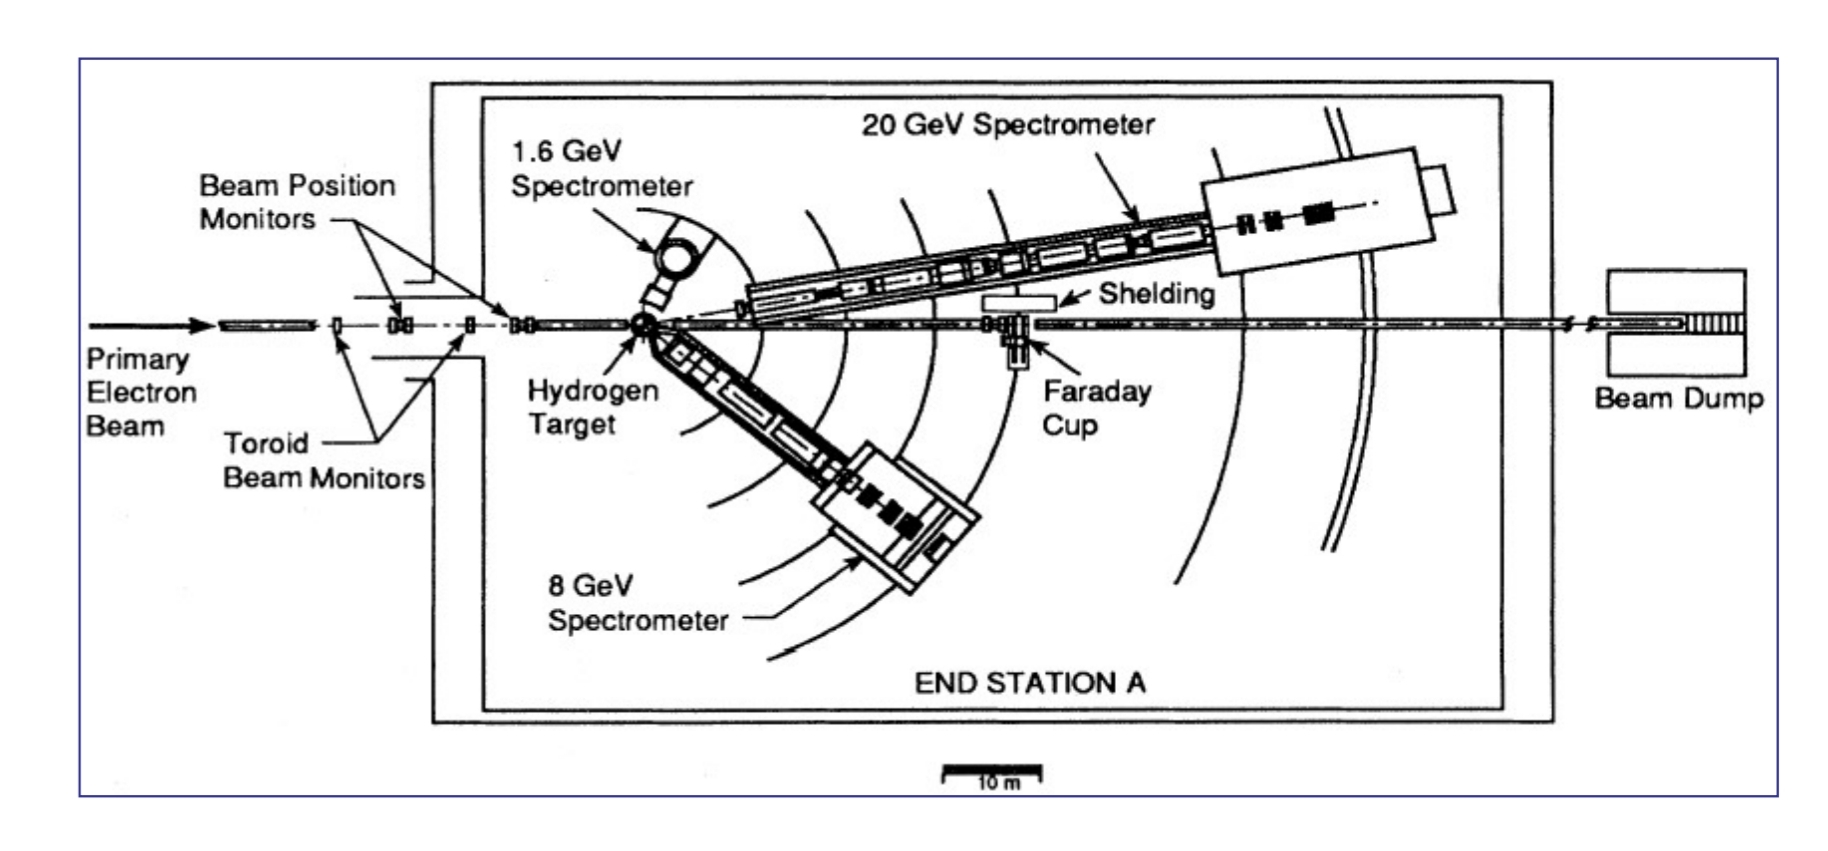
\includegraphics[scale=0.18]{Lezione18/gg.jpg} 
\end{figure}
Siccome la sezione d'urto, ricordo che quando abbiamo fatto la scomposizione della sezione d'urto in onde parziali avevamo visto che la sezione d'urto ha un limite superiore che va come $1/k^2$ quindi come uno su momento al quadrato della particella incidente. Quindi siccome siamo ad energie molto più alte la sezione d'urto è molto più bassa e quindi per avere un tasso di eventi importante bisogna utilizzare un bersaglio molto più "denso". Quindi il bersaglio al posto di essere idrogeno gassoso (come nell'esperimento di Hofstadter) ho idrogeno liquido. Sono necessarie tre diversi analizzatori magnetici per i diversi range di energia che vogliamo vedere. La Faraday Cup serve a misurare la carica che passa e quindi è un modo per normalizzare la sezione d'urto differenziale.
\subsection{Misura della sezione d'urto}
Queste sono le misure fatte. I grafici rappresentano la misura delle sezioni d'urto in funzione della massa del sistema adronico: $\sqrt{(p+q)^2}$. La procedura di misura quale è. Fisso l'energia dei fasci, fisso l'angolo in cui inserisco lo spettrometro e dopo cambiando il campo magnetico nel mio spettrometro vario l'energia $E'$ degli elettroni che riescono a superare lo spettrometro. Sono in grado di misurare il tasso di interazione degli elettroni con un $E'$ che varia tra l'energia di soglia dello spettrometro che è circa $3\,GeV$ e l'energia massima data dalla dormula di scattering. Quindi quando ho questa energia massima e minima posso coprire un range di momento trasferito:
\begin{equation*}
    4EE'_{\mathrm{min}}\sin^2{\frac{1}{2}\theta}<Q^2<4EE'_{\mathrm{max}}\sin^2{\frac{1}{2}\theta}
\end{equation*}
Se ad esempio prendo il primo grafico con elettroni a $7\,GeV$. Siamo in una regione in cui il $W$ massimo non è molto grande ma si notano benissimo le strutture di risonanza. Vedo che ho la produzione di questi stati eccitati. Quando aumento l'energia (aumento il $Q^2$) questa struttura delle risonanze in qualche modo tende a svanire. In dettaglio le scale vericale vediamo che le sezioni d'urto calano molto velocemente. Siamo in una regione in cui i fattori di forma sono molto importanti. Invece se andiamo a vedere la regione a grande massa. Quindi in urti profondamente anelastici e quindi dove ho trasferito molta energia al mio nucleo, ho creato degli stati adronici più complessi. Quello che si vede è che la sezione d'urto diminuisce ancora con l'energia ma con quel andamento uno su energia al quadrato che è tipico delle interazioni puntiformi. Quindi abbiamo una fenomenologia che è molto simile all'esperimento di Rutherford che ad un certo punto vediamo che lo scattering ad alto momento trasferito è soppresso meno di quello che mi aspetterei da un fattore di forma che dovrebbe abbassare e azerrare lo scattering ad alto momento trasferito. Questo è l'indice che sto vedendo qualcosa di elementare. Qualcosa di "duro" all'interno del mio bersaglio. Prima osservazione che ha suscitato grande interesse. 
%IMMAGINE ewe 
\begin{figure}[htp!]
  \centering
  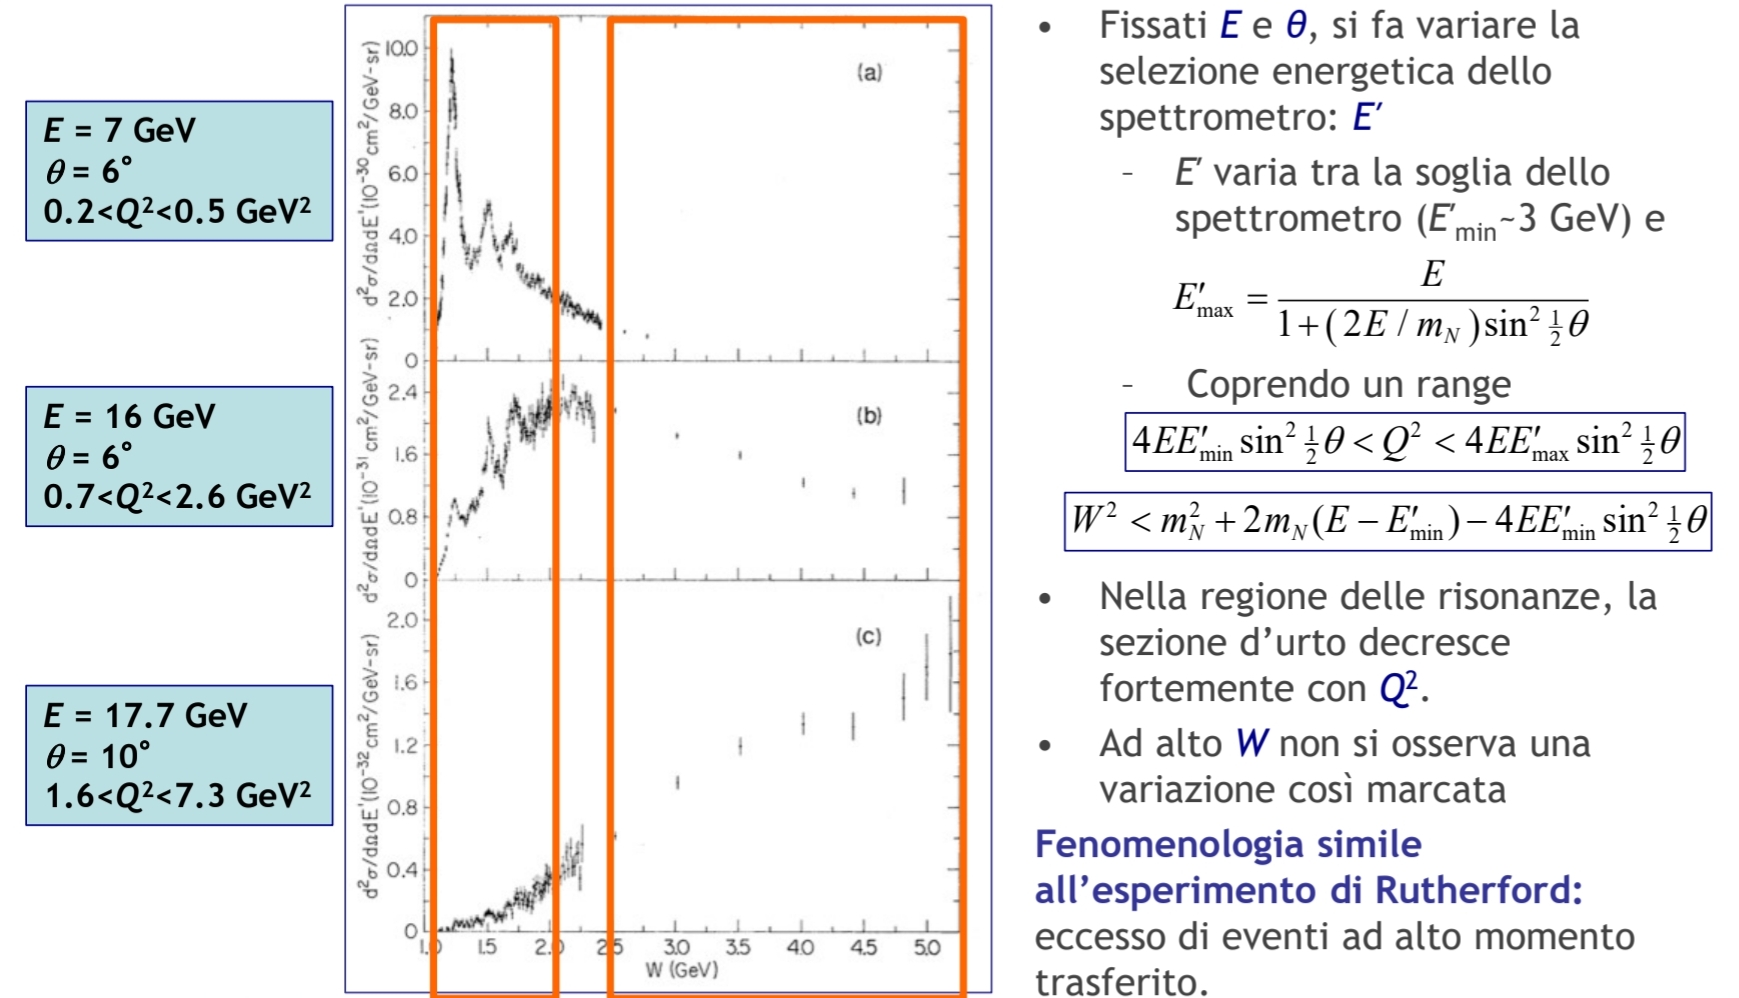
\includegraphics[scale=0.2]{Lezione18/ds.jpg} 
\end{figure}
\subsection{Funzioni di struttura}
L'altra cosa importante è che posso calcolarmi la funzione di struttura $F$ a partire dalla sezione d'urto. Facendo il rapporto tra la sezione d'urto che ho misurato e la sezione d'urto puntiforme che abbiamo visto. Posso fare il rapporto invertire la relazione e trovare $F_2$. $F_1$ è difficile da trovare perchè queste interazioni avvengono ad angoli piccoli e quindi riguardando la relazione il termine $\tan^2{\frac{1}{2}\theta}$ tende a zero. Quindi l'effetto di questo $F_1$ sono difficili da vedere. 
%IMMAGINE ewe 
\begin{figure}[htp!]
  \centering
  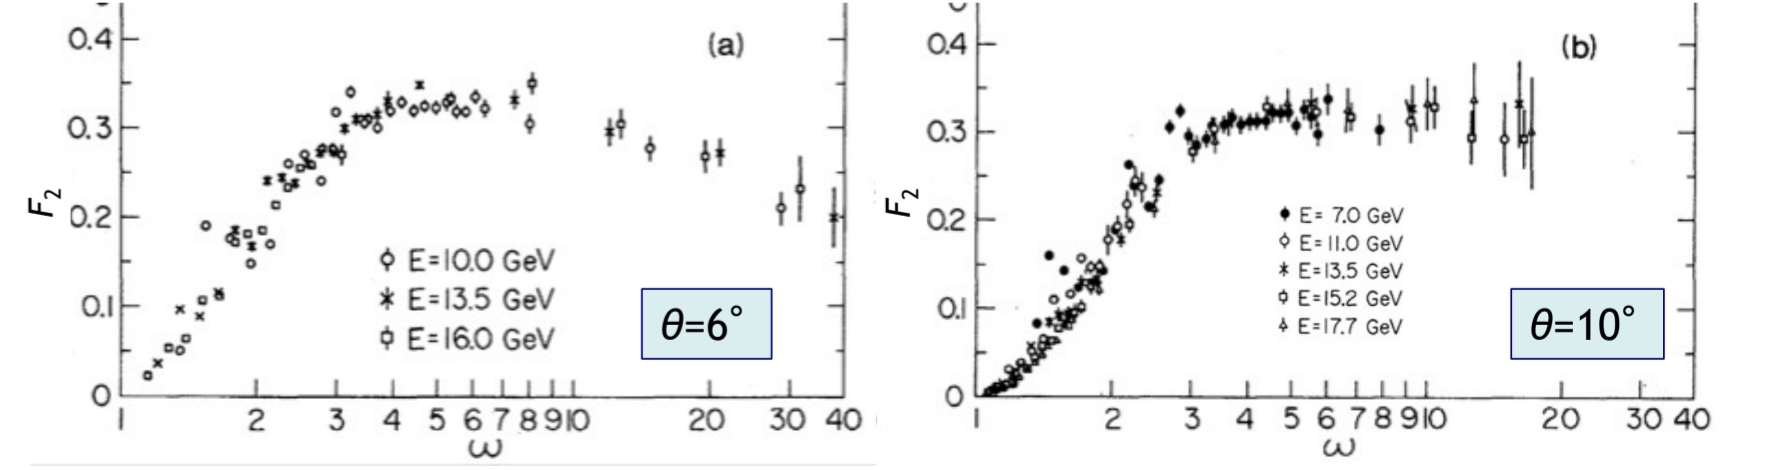
\includegraphics[scale=0.2]{Lezione18/dsa.jpg} 
\end{figure}
Questi due grafici sono quelli che contengono la scoperta dei quark anche se in maniera molto indiretta e non banale. Prima di tutto è notare che la variabile utilizzata è $\omega=1/x$. La cosa interessante è che se andiamo a vedere questi grafici abbiamo $F_2$ calcolato per lo stesso angolo ma diverse energie. Se prendiamo un $x$ fissato ($\omega$) e prendiamo $\theta$ fissato. Diverse energie dei fasci corrispondono di fatto a diversi valori di $Q^2$. Quindi questa curva è come se andassi a vedere in funzione della $x$ o della $\omega$ per diversi valori di $Q^2$. Quello che vediamo è che tutti i punti mirusati indipendentemente dall'energia del fascio sembrano stare sulla stessa curva. Quindi sembra quasi che $F_2$ non dipenda da $Q^2$ ma solo dalla $x$. Risultato importante (legge di scaling). Mi dice che il mio fattore di forma che dovrebbe dipendere sia da x che da Q dipende solo da x.
\subsection{Modello a partoni}
L'osservazione di questo particolare scaling e cioè che il fattore di forma dipende solo dalla $x$ lo posso spiegare se assumo che le interazioni che vedo tra l'elettrone e il protone (o nucleoni in generale), se assumo che lo scattering probabilmente inelastico invece sia uno scattering elastico con dei bersagli (quark) contenuto all'interno del nucleone. Per dimostrare questo c'è un conto un po' noioso ma i passi principali sono: consideriamo il caso di energie in gioco molto alte, in modo che si possa trascurare la massa del protone: $p^2\approx0$. Questo ad energie sempre più alte questa approssimazione è assolutamente buona. Introduciamo poi questa densità di probabilità $f_q(\xi)$ di trovare nel nucleone un quark $q$ con una frazione $\xi$ della quantità di moto del nucleone. La cosa interessante è che questo $\xi$ è una quantità misurabile perchè se dico che questo scattering è di tipo elastico tra l'elettrone e il quark bersaglio. Allora vale che la massa invariante del quark prima e dopo l'urto: 
\begin{equation*}
    (\xi p)^2=(\xi p+q)^2
\end{equation*}
Se ho questa uguaglianza trovo che questo $\xi$ è esattamente la variabile $x$ vista prima. Questa è una quantità che misuro dall'elettrone uscente. 

Se ho interazione con una particella puntiforme di spin $1/2$ allora la mia sezione d'urto sarà la sezione d'urto di Mott con la carica al quadrato del quark con cui sto interagendo (carica più alta interazione elettromagnetica più alta) moltiplicata poi per la sezione d'urto di Dirac per particelle puntiformi:
\begin{equation*}
    \left(\frac{d \sigma}{d \Omega}\right)_q(\xi)=\left(\frac{d \sigma}{d \Omega}\right)_{\text {Mott }} e_q^2\left[1+\frac{Q^2}{2 \xi^2 m_N^2} \tan ^2 \frac{1}{2} \theta\right]
\end{equation*}
Adesso però quello che vado a fare è che io vado a misurare nella forma doppio differenziale. E allora per scattering elastico abbiamo visto che il trucco è scrivere la sezione d'urto puntiforme per una $\delta$ che mi fissa l'$E'$ allo scattering elastico.
\begin{equation*}
    \left(\frac{d^2 \sigma}{d \Omega d E^{\prime}}\right)_q(\xi)=\left(\frac{d \sigma}{d \Omega}\right)_{\text {Mott }} e_q^2\left[1+\frac{Q^2}{2 \xi^2 m_N^2} \tan ^2 \frac{1}{2} \theta\right] \delta\left(E^{\prime}-E+\frac{Q^2}{2 \xi m_N}\right)
\end{equation*}
Il contributo di questo tipo di quark alla sezione d'urto totale si ottiene integrando i possibili valori di $\xi$, pesati con la rispettiva probabilità.
\subsection{Struttura del protone}
Dallo studio di diverse interazioni:
\begin{equation*}
    e+p, \quad e+n, \quad \mu^{\pm}+N
\end{equation*}
e altri si possono determinare le $f_q$ per i vari quark. Si trova in maniera consistente che le sezione d'urto: possono venire espresse in termini di sezioni d'urto elementari, pesate per le densità di probabilità dei quark interessati e per un dato adtrone sono universali e valide per tutti i processi. La struttura "partonica" del protone è molto più ricca di quanto ci si potrebbe aspettare: è definito il "contenuto di sapore" del protone:
%IMMAGINE ewe 
\begin{figure}[htp!]
  \centering
  
\includegraphics[scale=0.2]{Lezione18/uu.jpg} 
\end{figure}
quello che si vede è che a basso $x$ quindi in dimensioni molto piccole quello che abbiamo è che troviamo che nel protone troviamo anche una grande quantità di anti-quark. Ed in un protone che non ha stranezza troviamo anche una certa quantità di quark s e quindi la nostra struttura è molto dinamica. Quindi dentro il protone potenzialmetne ci sono tutti i tipi di quark ma quello che mi dice il modello a quark è che i numeri quantici del protone devono essere ben definiti. 
\begin{equation*}
    \int_0^1dx(f_u(x)-f_{\Bar{u}}(x))=2 \quad \int_0^1dx(f_d(x)-f_{\Bar{d}}(x))=1
\end{equation*}
Quindi il "numero totale" di quark cresce a x piccoli, esiste un contributo dovuto a particelle neutre: i gluoni. Il numero quantico di sapore che è alla base della formulazione SU(3) lo devo vedere non come rigidamente il protone costituito da 3 quark ma come uno stato costituito da distribuzioni di quark e anti-quark molto variegata e dinamica che dipende dalla scala di energia delle interazioni che posso vedere e non vedere però mantengono i numeri quantici. Un'altra cosa importante è che si vede anche la densità di probabilità di vedere un gluone (particella mediatrice delle interazioni forti). Ha una densità di probabilità molto alta all'interno del protone. All'interno del protone i quark sono immersi in un mare di gluoni che riescono a tenerli insieme. Questo è molto interessante perchè da l'idea che la struttura reale degli oggetti di cui abbiamo a che fare non è così banalmente riconducibile a particelle elementari. Si ritorna un pochino al concetto di equivalenza tra particelle e campo. In un certo senso il campo corrispondente all'up e all'anti-up ci sono entrambi nel protone ma hanno valori molto bassi a meno che io non vada a interazioni con scattering profondamente inelastici andando ad eccitare questi stati trasferendo energia e allora li riesco a vedere.
\subsection{Libertà asintotica e Confinamento}
La cosa interessante è che tutto questo discorso che abbiamo fatto sullo scaling dei fattori di forma e quindi che la $F$ dipende dalla $x$ ma non dal $Q^2$ abbiamo completamente trascurato le interazioni tra i quark all'interno degll'adrone. Con l'aggiunta del pezzo di Dirac abbiamo messo l'interazione tra quark e elettrone (spin $1/2$) ce ne siamo fregati delle possibili interazioni che possono avere tra di loro. Il fatto che questa approssimazione funzioni bene prende il nome di \textbf{libertà asintotica}. In prima approssimazione possiamo trascurare l'effetto delle interazioni forti quando vediamo scattering profondamente anelastici. Questa libertà asintotica ci fornisce una prova dell'esistenza dei quark come entità reali. Questo perchè vediamo che possiamo descrivere le interazione tra i quark con dei numeri quantici fissati. Sembra però in contraddizione con il fatto che i quark liberi non sono mai stati osservati ma solo in stati legati. Per quanto noi buttiamo elettroni con energia sempre più alta contro gli adroni non vediamo uscire quark. Vediamo uscire altri adroni. Questo fenomeno prende il nome di \textbf{confinamento}. Sembrano due fenomeni in contraddizione. Da una parte abbiamo una interazione che sembra essere trascurabile (quando vado a vedere i quark) che è l'interazione forte. Ma dall'altra parte è così forte che non mi permette ai quark di uscire dagli adroni. Come possono coesistere questi fenomeni?

\subsubsection{Confinamento: potenziale q-q}
Lo studio degli stati legati di quark pesanti permette di avere delle informazioni circa il potenziali quark-antiquark. Il modo classico di farlo è andare a vedere i livelli energetici degli stati legati quark-antiquark. Esattamente come avevamo fatto con il deutone: vedo che ho una certa energia di legame, so che la dimensione del sistema è questa quindi quanto deve essere profonda la buca di potenziale per darmi energia di legame giusta? In questo modo siamo riusciti a risalire dai livelli energetici a caratteristiche del potenziale.
%IMMAGINE ewe 
\begin{figure}[htp!]
  \centering
  
\includegraphics[scale=0.2]{Lezione18/tt.jpg} 
\end{figure}
Qui si possono vedere varie risonanze charm e anti-charm e di b e anti-b in cui ho i livelli energetici di questa risonanze con i vari diversi numeri quantici. Studiando e guardando questa struttura si può risalire al potenziale che mi genera questi livelli energetici. Le osservazioni fatte in questo sistema ci dicono che a distanze $\sim fm$ il potenziale è della forma:
\begin{equation*}
    V(r)\approx kr
\end{equation*}
Quindi un potenziale che cresce linearmente con la distanza quark-antiquark. Un potenziale che non è superiormente limitato. Per questo fatto non è possibile estrarre un quark da un adrone fornendogli un'energia maggiore di quella di legame perchè non ho un'energia di legame massima che posso sottrarre. Questo entra in qualche modo nel definirmi il confinamento. Nel caso di un'interazione fortemente anelastica, qualitativamente: il quark riceve un tetraimpulso che ne modifica la traiettoria. Man mano che si allontana l'energia potenziale cresce. Ad un certo punto è conveniente (energeticamente parlando) estrarre dal vuoto una coppia quark-antiquark e chiudere le linee di forza creando nuovi mesoni e barioni.
%IMMAGINE ewe 
\begin{figure}[htp!]
  \centering
  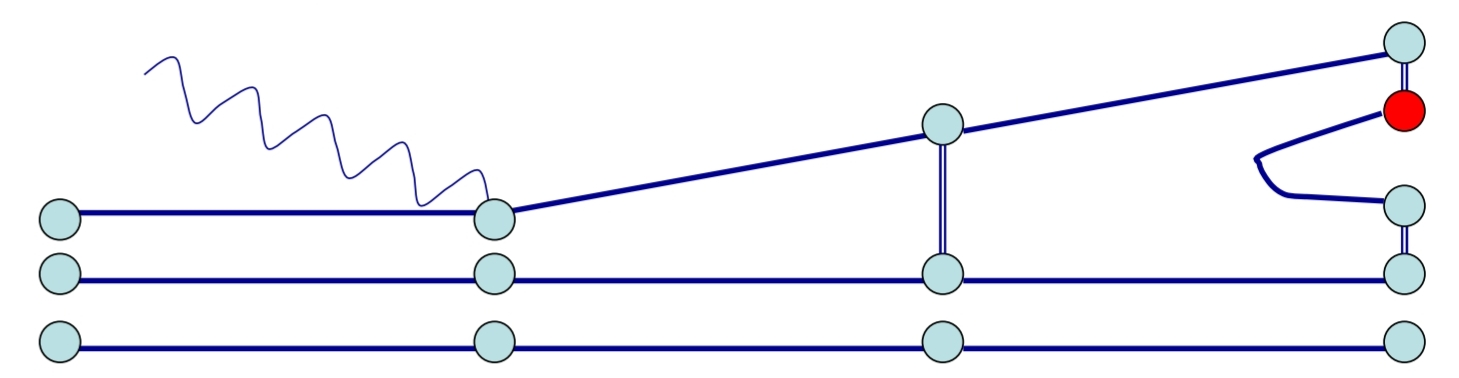
\includegraphics[scale=0.2]{Lezione18/yu.jpg} 
\end{figure}
Quindi sostanzialmente mi va a tagliare la "corda" che mi lega i due quark visto che l'energia potenziale cresce continuamente e mi va a creare una coppia quark  e anti quark che mi va a chiudere queste linee di energia potenziale. Se l'energia è molto grande anche dopo la prima rottura questo processo di disgregazione può continuare. Questo processo avviene su scale di lunghezza pari alle dimensoini degli adroni $\sim 1\,fm$ ed in tempi dell'ordine di $1\,fm/c=10^{-23,-24}s$
\subsubsection{Confinamento: getti}
Il processo di annichilazione $e^+e^-$ con produzione di adroni può venir trattato come produzione di una coppia di quark:
\begin{equation*}
    e^++e^-\to q+\Bar{q}
\end{equation*}
Ad alta energia il processo di stiramento delle linee di forza e loro taglio può avvenire multiple volte: si generano così getti di adroni.
\subsection{Il "colore"}
Dopo aver descritto le caratteristiche delle interazioni forti si pone il problema di definirne la natura. Deve esserci qualcosa di analogo ad una "carica" forte, che però non ha la stessa natura della carica elettromagnetica infatti questa "carica" genera un potenziale che cresce linearmente con la distanza. Questa "carica" deve anche permettere la creazione di stati "neturi" $q\Bar{q}$, $qqq$. Perchè se ci fosse il potenziale $kr$ non si creerebbe il nucleo. Il breve range delle forze nucleari è dovuto al fatto che due adroni devono avvicinarsi perchè i quark di uno vedano le cariche dell'altro. Fenomeno simile a quello degli atomi: a breve distanza possono interafire elettromagneticamente tramite forze di dipolo o di van der Waals, sebbene siano elettricamente neutri. Infatti dal punto di vista di forze nucleari il protone e il neutrone sarebbero neutri però quando vanno abbastanza vicini il quark del protone sente il quark del neutrone e viceversa e quindi c'è una interazione che quindi è a breve range. 
Un'altra cosa è l'evidenza di un grado di libertà interno ai quark. Può assumere tre stati diversi chiamato: \textbf{colore} per analogia al fatto che esistono tre colori fondamentali
\subsection{Evidenza del colore: i barioni}
%IMMAGINE ewe 
\begin{figure}[htp!]
  \centering
  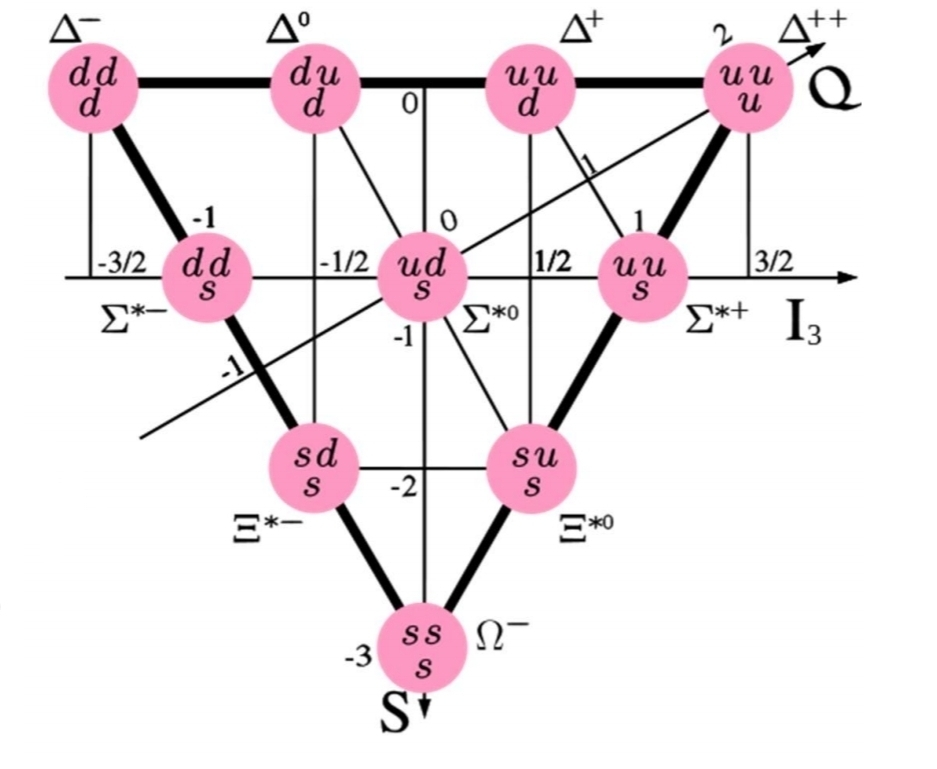
\includegraphics[scale=0.2]{Lezione18/ii.jpg} 
\end{figure}
Consideriamo il decupletto dei barioni è costituito da terne di quark nello stato fondamentale : $L=0$ e spin totale $=3/2$. I vertici del triangolo ($\Delta^-$, $\Delta^{++}$, $\Omega^-$) contengono risonanze con tre quark identici: la funzione d'onda deve essere anti-simmetrica per scambio di quark MA la funzione orbitale con $L=0$ è simmetrica, la funzione di spin, con tutti fli spin allineati a dare $3/2$ è pure simmetrica. Per cui per poter avere un'antisimmetria dobbiamo aggiungere qualcosa. Possiamo assumere che i quark possano esistere in tre stati di colore: r=red, g=green, b=blue, e costruire una combinazione antisimmetrica:
\begin{equation*}
    \Delta^{++}=\frac{1}{\sqrt{6}}(u_ru_gu_b+u_gu_bu_r+u_bu_ru_g-u_gu_ru_b-u_ru_bu_g-u_bu_gu_r)
\end{equation*}
Il grado di libertà interno si trasforma usando lo stesso gruppo di simmetria SU(3) usato per la simmetria di sapore. L'unica differenza è che ora gli operatori agiscono sul grado di libertà di colore invece che sul sapore dei quark. Gli stati neutri di colore sono quelli che non cambiano per trasformazione di colore. Nel caso dei mesoni lo stato neutro:
\begin{equation*}
    (q\Bar{q})=\frac{1}{\sqrt{3}}(q_r\Bar{q}_{\Bar{r}}+q_g\Bar{q}_{\Bar{g}}+q_b\Bar{q}_{\Bar{b}})
\end{equation*}
o detto anche bianco per usare la terminologia dei colori.

Un'altra evidenza sul colore è di tipo cinematico: il processo di annichilazione $e^+e^-$ per produrre una coppia fermione-antifermione nello stato finale è un processo elettromagnetico perchè mediato dalla carica di elettrone e antielettrone. L'intensità dipende dalla carica del fermione prodotto. Se $\sqrt{s}>>2m_f$ valgono le formule:
%IMMAGINE ewe 
\begin{figure}[htp!]
  \centering
  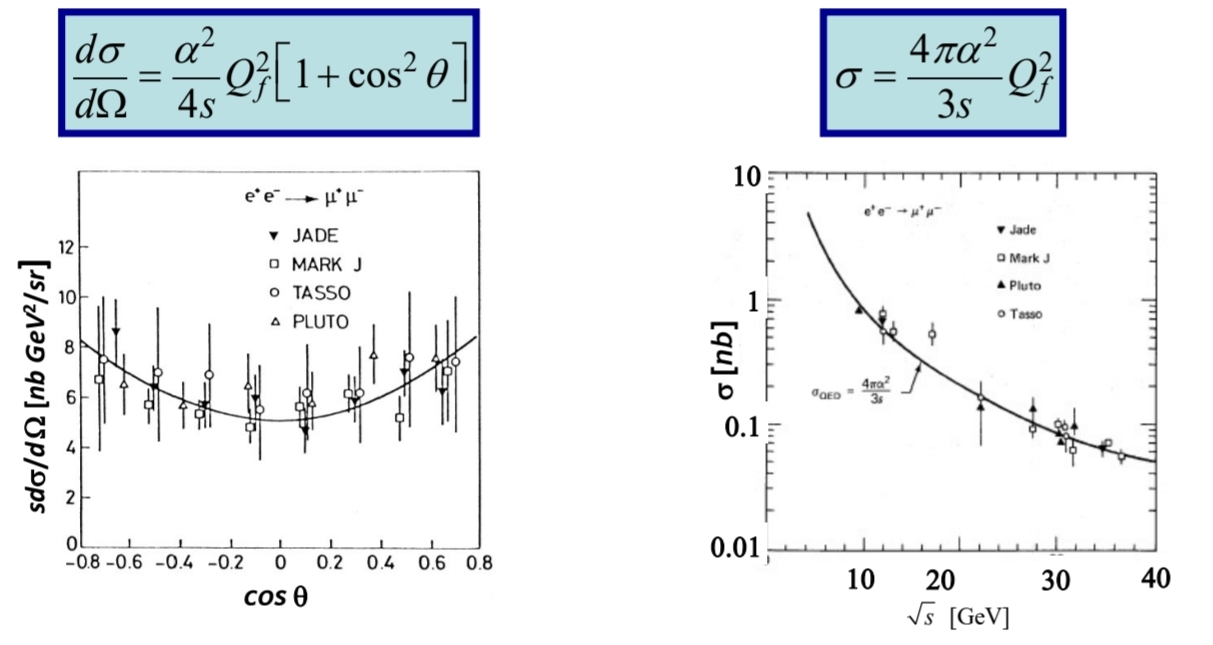
\includegraphics[scale=0.3]{Lezione18/yy.jpg} 
\end{figure}
Cosa succede se andiamo a vedere gli adroni? Il processo di annichilazione $e^+e^-$ per produrre adroni può venire interpretato come produzione di coppie quark-antiquark
%IMMAGINE ewe 
\begin{figure}[htp!]
  \centering
  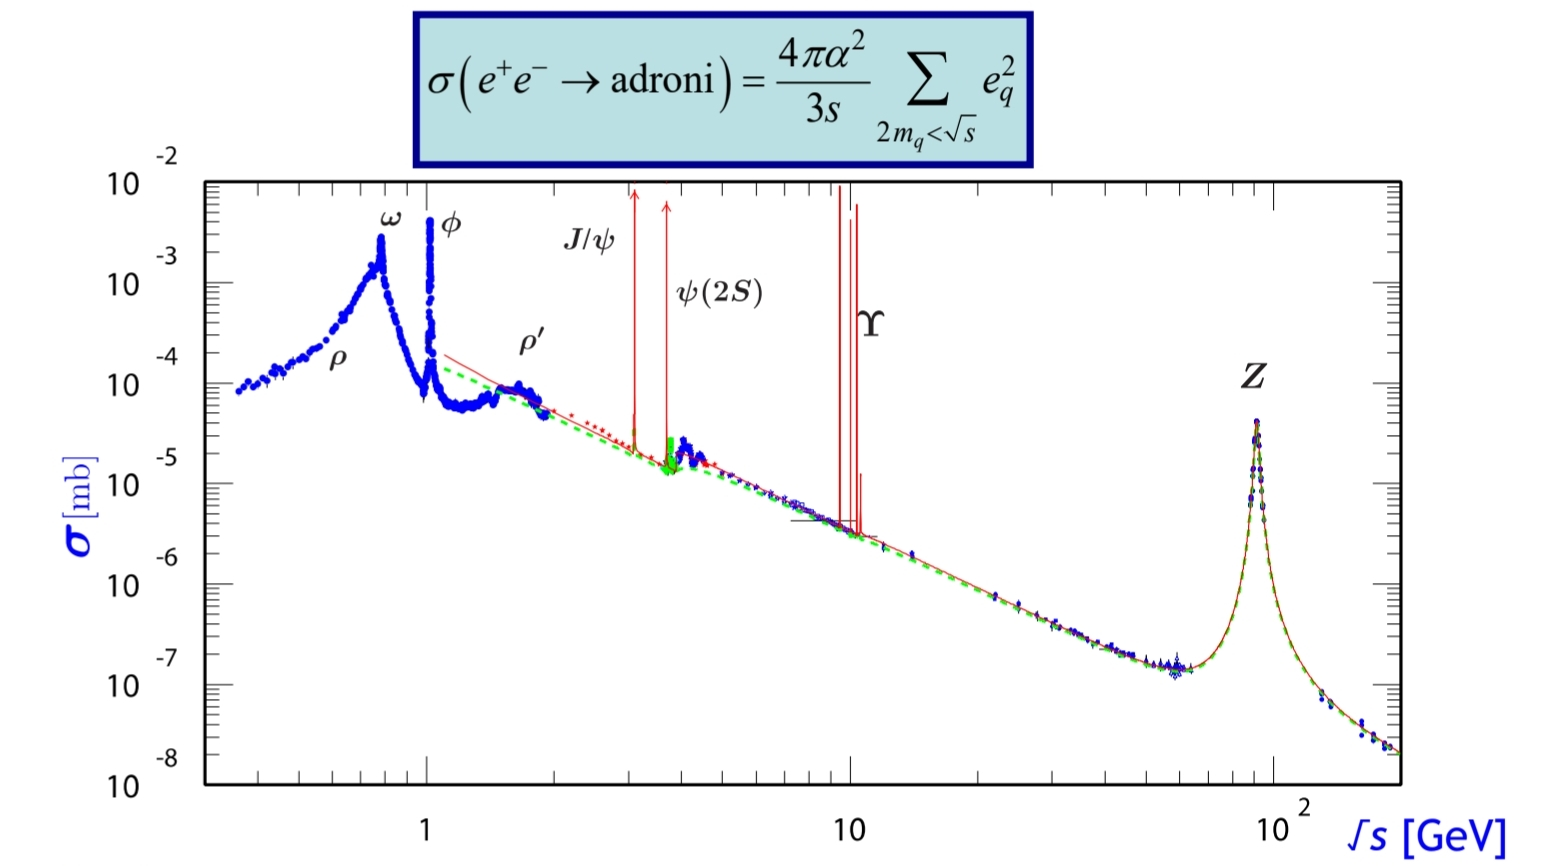
\includegraphics[scale=0.2]{Lezione18/ty.jpg} 
\end{figure}
Questo qui è il grafico in cui si vede in funzione della radice dell'energia del centro di massa la sezione d'urto. L'andamento è complesso perchè sono presenti molte risonanze però se si guardono le regioni tra le varie risonanze ci l'andamento è quello corretto però si vedono che queste rette sono un pochino sfalsate perchè vicino alla zona di risonanza in cui posso produrre la coppia quark-antiquark la sezione d'urto fa un salto dovuto al fatto che si aggiungono termini alla sommatoria.

Ora la cosa più semplice è andare a fare un rapporto:
\begin{equation*}
    R=\frac{\sigma(e^+e^-\to\text{adroni})}{\sigma(e^+e^-\to\mu^+\mu^-)}
\end{equation*}
Si fa questo perchè nello stesso esperimento posso miruare entrambe quindi facendo il rapporto si tolgono errori sistematici e successivamente è più comodo da visualizzare:
%IMMAGINE ewe 
\begin{figure}[htp!]
  \centering
  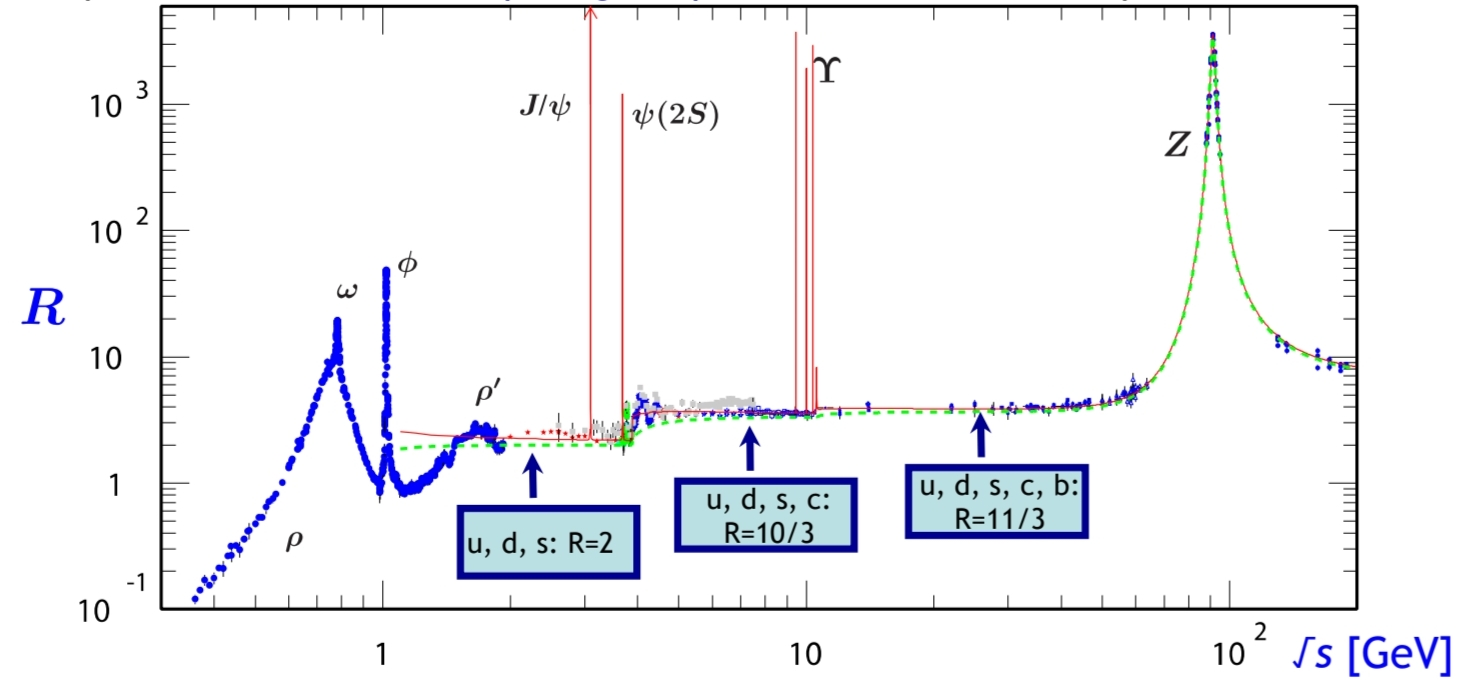
\includegraphics[scale=0.2]{Lezione18/ll.jpg} 
\end{figure}
Oltre a questo andamento si possono vedere le varie risonanze come gli stati legati bottom-antibotton lo stato legato charm-anticharm la $\phi$ che è uno stato legato $s$ e $\Bar{s}$ e poi sopra abbiamo la risonanza che corrisponde al bosone vettore delle interazioni deboli la $Z$. Quindi mi aspetto che questo rapporto $R$ sia la somma della carica al quadrato di tutti i quark possibili che posso produrre:
\begin{equation*}
    R=\frac{\sigma(e^+e^-\to\text{adroni})}{\sigma(e^+e^-\to\mu^+\mu^-)}=\sum_{2m_q<\sqrt{s}}e_q^2
\end{equation*}
Se vado sotto la soglia del charm (quindi nella posizione $R=2$) io mi aspetto che questa sommatoria sia:
\begin{equation*}
    \sum_{2m_q<\sqrt{s}}e_q^2=\frac{4}{9}+\frac{1}{9}+\frac{1}{9}=\frac{2}{3}
\end{equation*}
Dove la prima è la carica al quadrato del quark up, la seconda la carica al quadrato del quark down e la terza la carica del quark strange al quadrato. Quello che vedo sperimentalmente invece è che in questa regione la $R=2$ non $2/3$. Questo valore misurato me lo spiego se per ogni sapore ci sono tre diversi colori di quark. Allora la mia $R$ viene moltiplicata per il numero di colori:
\begin{equation*}
    R=\frac{\sigma(e^+e^-\to\text{adroni})}{\sigma(e^+e^-\to\mu^+\mu^-)}=N_{\text{colori}}\sum_{2m_q<\sqrt{s}}e_q^2
\end{equation*}
Visto che la mia coppia quark antiquark la posso creare con diverse combinazioni di colori mi ritrovo ad avere questo fattore. Questo fattore mi compensa il denominatore della sommatoria. Questo funziona anche per gli altri rapporti.
\subsection{I gluoni}
Se è valido il modello in cui le interazione equivalgono allo scambio di particelle mediatrici. Per cui abbiamo parlato di interazioni elettromagnetiche che avvengono con lo scambio di fotoni, le interazioni deboli abbiamo introdotto i bosoni $W$ e $Z$, scoperti poi al CERN. Abbiamo poi fatto il discorso sull'intensità delle forze dicendo che la massa di queste due particelle mediatrici deve essere intorno ai $100\,GeV$: $m_W=80\,GeV$ e $m_Z=90\,GeV$ è quella che da una parte produce il corto range delle interazioni deboli (intorno al millesimo di fermi) e viceversa giustifica anche le interazioni deboli siano effettivamente deboli. Questo perchè a bassa energia la particelle scambiata entra pesantemente a diminuirmi l'elemento di matrici. Se questo modello è valido devono esserci mediatori delle interazioni forti: i \textbf{gluoni}. Con le seguenti caratteristiche: devono essere neutri elettricamente e sono invece dotati di una carica di colore:
\begin{equation*}
    r\Bar{g}, \quad g\Bar{r}, \quad r\Bar{b},\quad b\Bar{r}, \quad g\Bar{b},\quad b\Bar{g}
\end{equation*}
incluse le varie combinazioni lineari:
\begin{equation*}
    \frac{1}{\sqrt{2}}(r\Bar{r}-g\Bar{g}),\quad \frac{1}{2}(r\Bar{r}+g\Bar{g}-2b\Bar{b})
\end{equation*}
Praticamente i quark sono colorati all'interno di un adrone, quello che fanno è scambiarsi dei gluoni per cambiare colore:
%IMMAGINE ewe 
\begin{figure}[htp!]
  \centering
  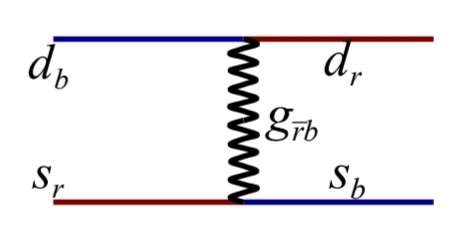
\includegraphics[scale=0.3]{Lezione18/col.jpg} 
\end{figure}
Una prima evidenza della presenza di gluoni nel prodone è data dalla frazione di momento trasportata dai quark. Se prendo la funzione di struttura $F_2$ che era data da $x$ (frazione di momento portata da un quark)per $f(x)$ che è la probabilità di trovare un quark con quel momento:
\begin{equation*}
    \frac{p_{\text{quark}}}{p_p}=\int dxF_2(x)=\int dx\sum_{q}xf_q(x)\approx\frac{1}{2}
\end{equation*}
Quindi questo integrale è la frazione di momento portata dai quark. Questa $F_2(x)$ si può misurare sperimentalmente. Il risultato è infatti che i quark portano solo la metà del momento del protone. Questo significa che deve esserci qualcosaltro che porta il momento del protone ma deve essere scarico altrimenti lo vedrei. Quindi metà del momento del protone è portato da particelle neutr, che contribuiscono a $F_2$.

Un'altra evidenza indiretta che questo passaggio è vero deriva dal fatto che il momento mancante venga portato da gluoni è confermato dalle sezioni d'urto in collisioni adroniche. La sezione d'urto di molti processi è dominata dalle collisione gluone-gluone. Esempio LHC:
\begin{equation*}
    \sigma(pp\to t\Bar{t})
\end{equation*}
La produzione di coppie top e anti-top. Riceve il contributo più importante dalla collisione di due gluoni:
\begin{equation*}
    \int_{x_{g1}x_{g2}>4m_t^2/s}dx_{g1}dx_{g2}f_g(x_{g1})f_g(x_{g2})\sigma(gg\to t\Bar{t})
\end{equation*}
Se tale termine non esistesse non si potrebbe avere accordo tra predizioni ed osservazioni sperimentali.
\subsection{Osservazione del gluone}
Anche il gluone, come per i quark, si pone il problema del confinamento. In collisioni ad alte energie può venir messa in evidenza la sua esistenza tramite il processo:
\begin{equation*}
    e^++e^-\to q+\Bar{q}+g
\end{equation*}
Avevamo visto che a collisioni a più o meno energia io producevo una coppia quark e antiquark con due getti che andavano in direzione opposta. Quello che può succedere che se ho tanta energia posso avere dei processi più complessi e produrre una terna. Come se uno di questi quark irraggiasse un gluone ad energia abbastanza alta da permettere al gluone di avere vita indipendente.
%IMMAGINE ewe 
\begin{figure}[htp!]
  \centering
  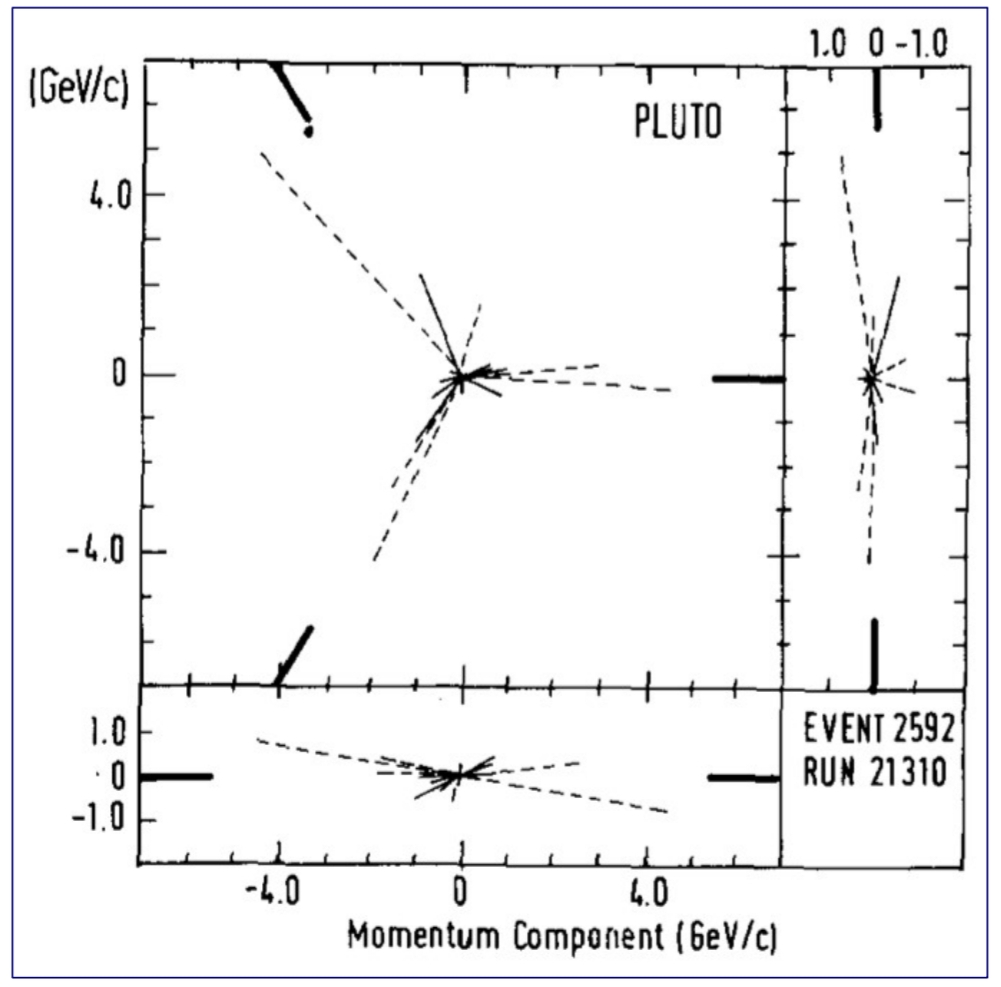
\includegraphics[scale=0.3]{Lezione18/tu.jpg} 
\end{figure}
In questo grafico la lunghezza di una linea corrisponde alla quantità di moto di una particella e poi in nero le linee continue sono particelle cariche, quelle tratteggiate neutre. Quello che si vede è che gli adroni non vengono prodotti in una configurazione a 2 getti ma in 3 getti. Questi sono coplanari e questo è quello che ci aspettiamo in un processo di produzione di 3 particelle. Il momento totale si deve annulare quindi si distribuiscono come un triangolo su un piano. Questa è la cosa più vicina all'osservazione diretta di un gluone. 

Ricapitolando abbiamo visto un insieme di evidenze del fatto che per le interazioni forti noi possiamo legarle alla presenza di un grado di libertà interna dei quark e possiamo descriverla attraverso lo scambio di gluoni come particelle mediatrici di questa interazione forte. Questa è la descrizione elementare delle interazioni forti. Poi si traduce invece in interazioni forti a livello nucleare come dovuta al fatto che gli adroni che sono costituiti da insieme di quark sono stati neutri secondo le interazioni forti ma quando due adroni si avvicinano sufficientemente allora i partoni di uno sentono i partoni dell'altro, possono interagire e questo è quello che mi genera le interazioni a breve range che troviamo all'interno dei nuclei tra protoni o tra protoni e pioni nelle interazioni nucleari a basse energie. 